\input{preamble}

\title{Section 1.5 --- Linear Functions --- Answer Key}

\newlength{\lwid}
\newlength{\lht}

\newcommand{\Lcirc}[1]{%
\setlength{\lwid}{\widthof{$#1$}}
\setlength{\lht}{\heightof{$#1$}}
\begin{tikzpicture}[baseline=0]
\useasboundingbox (-0.5\lwid,0) rectangle (0.5\lwid,\lht);
\draw (0,0) node[anchor=base]{$#1$};
\draw (0,0.5\lht) circle (1.75ex);
\end{tikzpicture}%
}

\newcommand{\CircBy}{
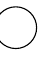
\begin{tikzpicture}[baseline=0]
\useasboundingbox (0,0) rectangle (0,1ex);
\draw (-1ex,1ex) circle (1.75ex);
\end{tikzpicture}%
}

\begin{document}
\maketitle

\section{Identifying Linear Expressions, Equations, and Functions}
Identify each expression as linear or not linear. If the expression is not linear, mark any parts of the expression that make it not linear.
\begin{smenum}
\mitemxxxx
{Linear}
{$\dfrac{3x-2}{\Lcirc{4x}+1}$}
{$\Lcirc{x^2}+2x+5$}
{Linear}
\end{smenum}
Identify each equation as linear or not linear. If the equation is not linear, mark any parts of the equation that make it not linear.
\begin{smenum}
\mitemxxxx
{$(\Lcirc{5x}+2)(\Lcirc{3x}-1)=14$}
{$\sqrt{\CircBy x+2}=x-4$}
{Linear}
{Linear}
\end{smenum}
Identify each function as linear or not linear. If the function is not linear, mark any parts of the function that make it not linear.
\begin{smenum}
\mitemxxxx
{Linear}
{$f(x)=3x+\Lcirc{x^3}$}
{$f(x)=\Abs{\CircBy 4x-3}$}
{Linear}
\end{smenum}

\section{Writing Linear Functions from Graphs}
For each function graphed below:
\begin{clist}
\item Write an equation for the function in point-slope form, using a point other than the y-intercept. Use $f$ as the name of the function.
\item Simplify your answer to give the function in slope-intercept form.
\item Give the coordinates of the line's $y$-intercept. Use your equation from part (b) if it is not clear on the graph.
\end{clist}
\begin{smenum}
\mitemxx
{
a. $f(x)=-\frac{4}{3}(x-3)-2$\\
b. $f(x)=-\frac{4}{3}x+2$\\
c. $(0,2)$
}{
a. One of two equations:\\$f(x)=\frac{3}{5}(x+3)+1$\\$f(x)=\frac{3}{5}(x-2)+4$\\
b. $f(x)=\frac{3}{5}x+\frac{14}{5}$\\
c. $(0,\frac{14}{5})$
}
\end{smenum}

\clearpage
\section{Graphing Linear Functions}
For each function below:
\begin{clist}
\item Fill in the table to show three points on the graph with integer coordinates.
\item Use two of your points to graph the function.
\item Confirm that the graph passes through the third point.
\end{clist}
\textbf{Note: If you were using the technique shown in the videos, you should have exactly the three points shown in the answer key.}
\begin{senum}
\item \begin{ilpic}[x=0.2in,y=0.2in]
\useasboundingbox (0,9) rectangle (1,-3);
\draw (0,5) node[anchor=south west]{$f(x)=\frac{3}{4}x-1$};
\draw (0,4) rectangle (10,0);
\draw (3,4) -- (3,0);
\foreach \y in {3,2,1} \draw (0,\y) -- (10,\y);
\foreach \x/\lbl in {1.5/x,6.5/y=f(x)} \draw (\x,3.2) node[anchor=base]{$\lbl$};
\foreach \y/\xlbl/\ylbl in {3/-4/-4,2/0/-1,1/4/2} {
	\draw (1.5,\y-0.8) node[anchor=base]{$\xlbl$};
	\draw (6.5,\y-0.8) node[anchor=base]{$\ylbl$};
}
\begin{scope}[xshift=6*0.2in+0.5\linewidth,yshift=3*0.2in]
	\DrawGridSquare
	\foreach \x/\y in {-4/-4,0/-1,4/2} \filldraw (\x,\y) circle (0.1);
	\linepoints(-5,-5)(5,5)(-4,-4)(0,-1)
\end{scope}
\end{ilpic}
\item \begin{ilpic}[x=0.2in,y=0.2in]
\useasboundingbox (0,9) rectangle (1,-3);
\draw (0,5) node[anchor=south west]{$f(x)=-\frac{3}{2}(x-2)+3$};
\draw (0,4) rectangle (10,0);
\draw (3,4) -- (3,0);
\foreach \y in {3,2,1} \draw (0,\y) -- (10,\y);
\foreach \x/\lbl in {1.5/x,6.5/y=f(x)} \draw (\x,3.2) node[anchor=base]{$\lbl$};
\foreach \y/\xlbl/\ylbl in {3/0/6,2/2/3,1/4/0} {
	\draw (1.5,\y-0.8) node[anchor=base]{$\xlbl$};
	\draw (6.5,\y-0.8) node[anchor=base]{$\ylbl$};
}
\begin{scope}[xshift=6*0.2in+0.5\linewidth,yshift=3*0.2in]
	\DrawGridSquare
	\foreach \x/\y in {0/6,2/3,4/0} \filldraw (\x,\y) circle (0.1);
	\linepoints(-5,-5)(5,5)(2,3)(4,0)
\end{scope}
\end{ilpic}
\end{senum}
\section{Inverses of Linear Functions}
Find the inverse of each linear function below. Show your work carefully on a separate sheet of paper.
\begin{smenum}
\mitemxxx
{$f\inv(x)=\frac{1}{2}x+4$}
{$g\inv(x)=\frac{7}{2}x-21$}
{$h\inv(x)=-\frac{3}{4}x+\frac{3}{2}$}
\mitemxxx
{$k\inv(x)=-\frac{1}{3}x-\frac{5}{3}$}
{$p\inv(x)=2x-6$}
{$q\inv(x)=\frac{9}{7}x-\frac{162}{7}$}
\end{smenum}
\end{document}